\section{Process and Outcome Reward Models}

\begin{frame}{}
    \LARGE Advanced Reasoning: \textbf{Process vs Outcome Reward Models}

    \vspace{1em}
    \normalsize Should a scorer judge the final answer or every step, and what happens when a policy trains against it?
\end{frame}

\begin{frame}{Four Kinds of Scorer}
    \begin{center}
    \small
    \renewcommand{\arraystretch}{1.05}
    \begin{adjustbox}{max width=\linewidth}\begin{tabular}{>{\raggedright\arraybackslash}p{3.6cm}>{\raggedright\arraybackslash}p{4.6cm}>{\raggedright\arraybackslash}p{5.4cm}}
        \toprule
        \textbf{Model} & \textbf{Predicts} & \textbf{Trained with} \\
        \midrule
        Preference reward model (RLHF) & one scalar per sequence & pairwise loss on human comparisons \\
        \textbf{Outcome reward model (ORM)} & is the final answer correct? & binary cross-entropy on the outcome label \\
        \rowcolor{KAUSTcyan!12} \textbf{Process reward model (PRM)} & is each \emph{step} correct? & per-step labels at step delimiters \\
        Value function & expected remaining return & regression on on-policy rollouts \\
        \bottomrule
    \end{tabular}\end{adjustbox}
    \end{center}
    \vspace{-0.3em}
    \[
        \mathcal{L}_{\text{ORM}} = y_s \log r_s + (1-y_s)\log(1-r_s)
        \qquad
        \mathcal{L}_{\text{PRM}} = \sum_{i=1}^{K} y_{s_i}\log r_{s_i} + (1-y_{s_i})\log(1-r_{s_i})
    \]
    \begin{itemize}\itemsep0.3em
        \item A PRM gives $K$ scores per solution. To rank solutions, reduce them to one: \textbf{product}, \textbf{minimum} or \textbf{last step}. The best choice depends on where the labels came from.
    \end{itemize}
    \src{Lambert, RLHF book, reward modelling chapter (accessed Oct 2026). Losses as in Wang et al., ``Math-Shepherd,'' \href{https://arxiv.org/abs/2312.08935}{arXiv:2312.08935}.}
\end{frame}

\begin{frame}{The Classic Result: Verify Step by Step}
    \begin{columns}[T,onlytextwidth]
        \column{0.45\textwidth}
        \centering
        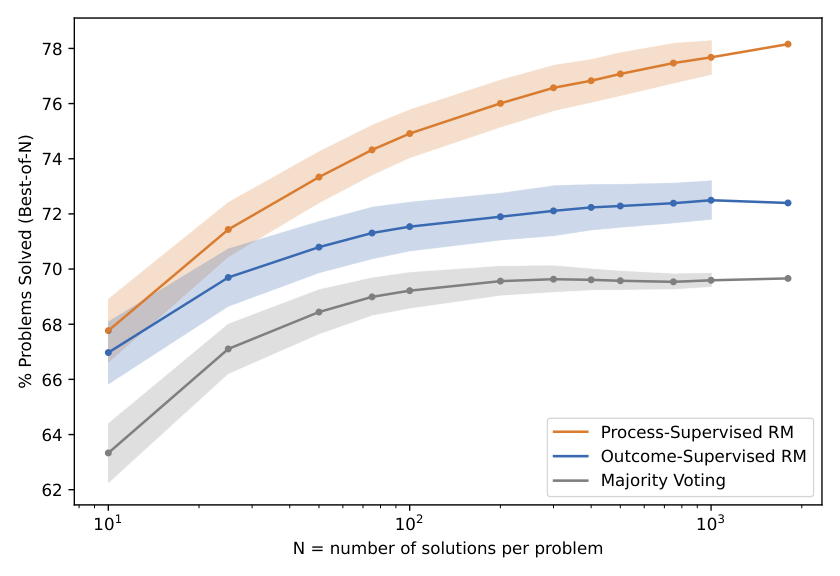
\includegraphics[width=\linewidth,height=0.6\textheight,keepaspectratio]{images/advanced-reasoning/lightman_fig3_prm_orm_bon.png}
        \column{0.53\textwidth}
        \begin{itemize}\itemsep0.45em
            \item \textbf{PRM800K:} about 800,000 human labels on the steps of 75,000 solutions to 12,000 MATH problems.
            \item \textbf{Best-of-1860 on MATH:} PRM 78.2\%, ORM 72.4\%, majority vote 69.6\%. The PRM curve is still rising where the others are flat.
            \item \textbf{Out of distribution} (recent AP and AMC exams): 72.9, 63.8 and 61.3.
            \item \textbf{Active learning} made labelling about 2.6$\times$ more efficient. Annotators saw mostly ``convincing wrong-answer'' solutions.
        \end{itemize}
    \end{columns}
    \vspace{0.1em}
    \src{Lightman et al. (OpenAI), ``Let's Verify Step by Step,'' \href{https://arxiv.org/abs/2305.20050}{arXiv:2305.20050}, Figure 3 and Table 1.}
\end{frame}

\begin{frame}{Step Labels Without Humans}
    \begin{itemize}\itemsep0.35em
        \item Human step labels do not scale. \textbf{Monte Carlo labels:} from step $s_i$, sample $N$ completions and check their answers $a_j$ against the truth $a^*$:
        \[
            y^{\text{hard}}_{s_i}=\mathbb{1}\big[\exists\, j:\ a_j=a^*\big]
            \qquad
            y^{\text{soft}}_{s_i}=\frac{1}{N}\sum_{j=1}^N\mathbb{1}[a_j=a^*]
        \]
        \item \alert{What this actually measures.} Not whether the step is valid, but whether \emph{this completer} can finish from here. It is a value estimate.
        \item \textbf{Implicit PRM:} no step labels at all. Train on outcomes with $r_\theta(\mathbf{y})=\beta\log\frac{\pi_\theta(\mathbf{y})}{\pi_{\text{ref}}(\mathbf{y})}$. Its partial sums are Q-values, and their increments are step rewards.
        \item \textbf{PRIME} trains policy and implicit PRM together, online. A \emph{static} PRM decays from about 75\% to 45\% accuracy as the policy moves.
    \end{itemize}
    \src{Wang et al., ``Math-Shepherd,'' \href{https://arxiv.org/abs/2312.08935}{arXiv:2312.08935}. Yuan et al., ``Free Process Rewards without Process Labels,'' \href{https://arxiv.org/abs/2412.01981}{arXiv:2412.01981}. Cui et al., ``PRIME,'' \href{https://arxiv.org/abs/2502.01456}{arXiv:2502.01456}.}
\end{frame}

\begin{frame}{Is Your PRM a Process Model, or an Outcome Judge in Disguise?}
    \begin{columns}[T,onlytextwidth]
        \column{0.47\textwidth}
        \centering
        \begin{adjustbox}{max width=\linewidth}\begin{tikzpicture}
            \begin{axis}[xbar, width=4.9cm, height=5.6cm, bar width=0.3cm,
                xmin=0, xmax=112, xlabel={\scriptsize ProcessBench average F1},
                symbolic y coords={Math-Shepherd PRM,PRM800K PRM,Llama-3.3-70B,GPT-4o,QwQ-32B-Preview,o1-mini}, ytick=data,
                y tick label style={font=\scriptsize}, x tick label style={font=\scriptsize},
                nodes near coords, nodes near coords style={font=\tiny},
                axis lines=left, enlarge y limits=0.12]
                \addplot[fill=KAUSTcyan!55, draw=KAUSTcyan!70!black] coordinates {(31.5,Math-Shepherd PRM) (56.5,PRM800K PRM) (58.0,Llama-3.3-70B) (61.9,GPT-4o) (71.5,QwQ-32B-Preview) (87.9,o1-mini)};
            \end{axis}
        \end{tikzpicture}\end{adjustbox}

        {\scriptsize Task: find the earliest wrong step in 3,400 solutions}
        \column{0.5\textwidth}
        \begin{itemize}\itemsep0.4em
            \item Best-of-N rewards a PRM for guessing the \emph{outcome}. \textbf{ProcessBench} asks the real question: where is the first error?
            \item Trained PRMs \alert{trail prompted critics}. By label source: human 56.5, LLM judge 46.5, Monte Carlo 40.1.
            \item \textbf{Process-to-outcome drift.} For several PRMs, over 40\% of minimum scores fall on the \emph{final} step.
            \item That explains the reductions. Monte Carlo PRMs work best with ``last step''. Human-labelled ones with product or minimum.
        \end{itemize}
    \end{columns}
    \vspace{0.1em}
    \src{Zheng et al. (Qwen), ``ProcessBench,'' \href{https://arxiv.org/abs/2412.06559}{arXiv:2412.06559}. Zhang et al. (Qwen), ``The Lessons of Developing Process Reward Models in Mathematical Reasoning,'' \href{https://arxiv.org/abs/2501.07301}{arXiv:2501.07301}, Tables 4 and 5.}
\end{frame}

\begin{frame}{Verification as Generation}
    \begin{itemize}\itemsep0.4em
        \item A discriminative PRM is a classifier with fixed compute. Why not let the verifier \emph{think}?
        \item \textbf{Generative verifier (GenRM).} Ask ``Is the answer correct?'' and read the probability of ``Yes''. With verification chains $v^{(i)}$, average over $K$ of them:
        \[
            r_{\text{MajV@}K}(x,y)=\frac{1}{K}\sum_{i=1}^{K}p_\theta\big(\text{Yes}\mid x,y,v^{(i)}_{\text{CoT}}\big)
        \]
        Accuracy rises with $K$. \textbf{The verifier has its own test-time scaling.}
        \item \textbf{ThinkPRM.} Fine-tune a reasoning model on about 1,000 verification chains. It beats discriminative PRMs trained on 712,000 labels, about 100$\times$ more.
        \item \textbf{In production recipes.} Kimi k1.5 compared a value-head reward model with a chain-of-thought one on spot checks: 84.4\% against 98.5\%. The second went into RL.
    \end{itemize}
    \vspace{0.05em}
    \src{Zhang et al., ``Generative Verifiers,'' ICLR 2025, \href{https://arxiv.org/abs/2408.15240}{arXiv:2408.15240}. Khalifa et al., ``Process Reward Models That Think,'' \href{https://arxiv.org/abs/2504.16828}{arXiv:2504.16828}. Kimi Team, \href{https://arxiv.org/abs/2501.12599}{arXiv:2501.12599}.}
\end{frame}

\begin{frame}{Inside RL, Outcome Rewards Won}
    \begin{itemize}\itemsep0.3em
        \item A denser reward should help. Why did DeepSeek-R1 and Kimi k1.5 refuse PRMs? Steps are hard to define and judge, and:
        \begin{itemize}\itemsep0.1em
            \item a model-based reward invites \alert{reward hacking}
            \item a wrong step followed by recovery is useful exploration. Per-step credit would punish it
        \end{itemize}
    \end{itemize}
    \begin{center}
    \small
    \renewcommand{\arraystretch}{1.12}
    \begin{adjustbox}{max width=\linewidth}\begin{tabular}{>{\raggedright\arraybackslash}p{4.4cm}>{\raggedright\arraybackslash}p{9.4cm}}
        \toprule
        \textbf{Use of the process signal} & \textbf{What happened} \\
        \midrule
        Added to the reward & entropy collapses, responses grow and repeat. Ends \emph{below} plain GRPO (47.3 against 49.9) \\
        Policy trained against a PRM & PRM reward above 0.9 while true accuracy stays below 4\% \\
        \rowcolor{KAUSTcyan!12} As a data filter (PROF) & drop samples where process and outcome disagree. 51.7 against 49.9 \\
        \rowcolor{KAUSTcyan!12} Online and implicit (PRIME) & the scorer moves with the policy \\
        \bottomrule
    \end{tabular}\end{adjustbox}
    \end{center}
    \vspace{-0.2em}
    \takeaway{For Day 3: under mild assumptions, GRPO with an outcome reward \emph{already is} a Monte Carlo PRM.}
    \src{DeepSeek-AI, \href{https://arxiv.org/abs/2501.12948}{arXiv:2501.12948}. Kimi Team, \href{https://arxiv.org/abs/2501.12599}{arXiv:2501.12599}. Ye et al. (PROF), \href{https://arxiv.org/abs/2509.03403}{arXiv:2509.03403}, Table 2. Tiwari et al., ``Reward Under Attack,'' \href{https://arxiv.org/abs/2603.06621}{arXiv:2603.06621}. Sullivan and Koller, ``GRPO is Secretly a Process Reward Model,'' \href{https://arxiv.org/abs/2509.21154}{arXiv:2509.21154}.}
\end{frame}

\begin{frame}{Reward Models: What to Remember}
    \begin{itemize}\itemsep0.4em
        \item \textbf{For selection at inference}, process models beat outcome models and votes. But best-of-N alone is a biased way to measure a PRM.
        \item \textbf{Monte Carlo step labels estimate a value}, not logical validity. Check which one your PRM learned.
        \item \textbf{Generative verifiers} are replacing discriminative ones. They need far fewer labels and scale with compute.
        \item \textbf{As an RL reward}, a static learned PRM gets hacked. Verifiable outcome rewards stay the anchor.
    \end{itemize}
    \vspace{0.1em}
    \begin{block}{State of play, October 2026}
        No public source shows a frontier lab using a learned PRM as the RL reward of a production model.
    \end{block}
    \vspace{0.3em}
    \takeaway{\textbf{Next.} A learned scorer can always be fooled. An interpreter cannot. What if part of the reasoning is \emph{executed} instead of judged?}
\end{frame}
